\section[EVOLUTIONARY DUNGEON DESIGNER]{EVOLUTIONARY DUNGEON \\DESIGNER}

This section presents the~\acrfull{edd} research tool, all its features, and the multiple interactions between the human designer and the AI. First, it describes the tool's objectives, the iterations it has gone through, and game design patterns as a significant feature. Then, it presents and discusses the room generation process and multiple designer interactions. Finally, it describes the tool's workflow.

% \begin{itemize}
%     \item Total description of EDD, and what it enables
%     \item workflow and development
% \end{itemize}

\begin{figure}[!h]
\centerline{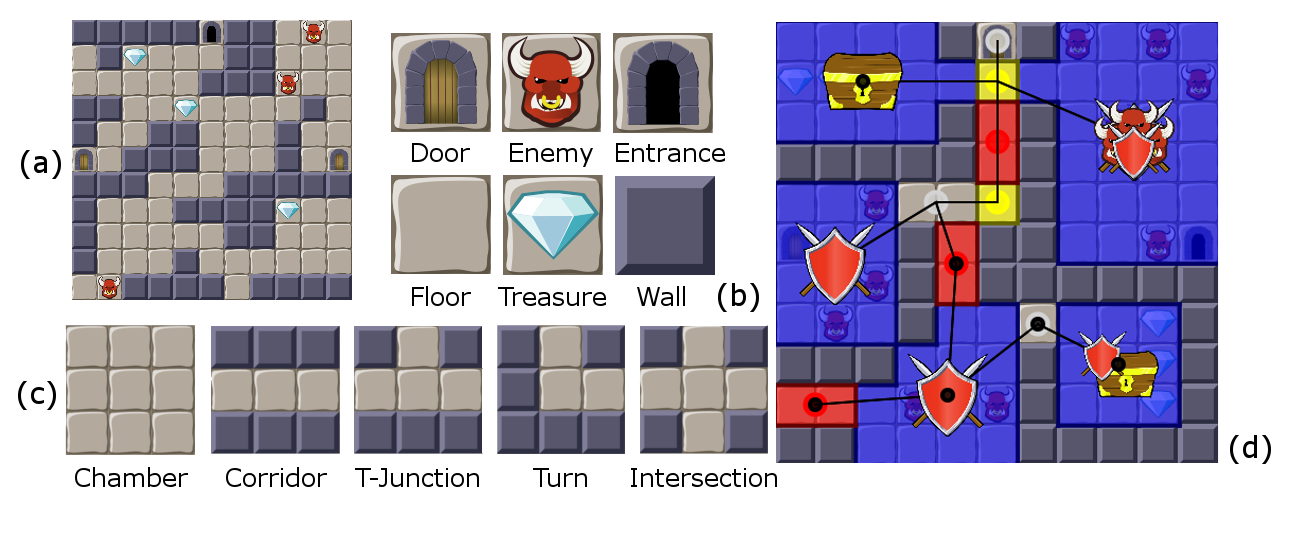
\includegraphics[width=\textwidth]{figures/EDD-figs/map-figure.png}}
\caption{Main components in EDD. (a) Basic example room, (b) different placeable tiles (the boss tile looks the same as the enemy tile but 3 times bigger), (c) spatial-patterns and (d) meso-patterns} \label{fig:tilesPats}
\end{figure}

The~\acrshort{edd} is an~\acrshort{micc} system to create dungeons for rogue-like and adventure games, similar to the ones found in Zelda~\cite{tloz} or the Binding of Isaac~\cite{bindingISAAC}. The main feature of~\acrshort{edd} is the collaboration between designer and computational designer to create rooms. The designer focuses on editing the room to design their goals. In parallel, they are continuously offered a set of suggestions adapted to their current design, which they can use. In addition, the designer's design is continuously evaluated for design patterns, feasibility and playability constraints, and enhanced information of the rooms such as door safety or enemy-treasure balance. This information is given to the designer at different time steps to help them develop their design.

% the designer is provided with additional information

The first iteration of~\acrshort{edd} was described and presented by Baldwin et al.~\cite{baldwin_mixed-initiative_2017,baldwin_towards_2017}. In their work, the aim was on creating the first steps towards a~\acrshort{micc} system that allowed the designer to create fixed-sized individual rooms while being suggested four generated rooms by request. Furthermore,~\acrshort{edd} was developed further with a revamped UI, allowing the creation of complete dungeons, and providing augmented information on the suggestions compared to the current design~\cite{alvarez_fostering_2018,alvarez_assessing_2018}. Finally, the latest version of~\acrshort{edd} is the one presented on this thesis, which incorporates the~\acrshort{icmape} and allows the designer to create dungeons in whatever layout preferred~\cite{alvarez_empowering_2019,alvarez_interactive_2020}. In addition,~\acrshort{edd} now includes prototype implementations of different designer models: the designer preference model~\cite{alvarez_exploring_2020} and designer personas~\cite{alvarez_designer_2022}.

Dungeons in~\acrshort{edd} are an acyclical graph composed of interconnected rooms. Rooms are a rectangular $M \times N$ grid of tiles, which might be: \emph{Floor}, \emph{Wall}, \emph{Treasure}, \emph{Enemy}, \emph{Enemy Boss}, and \emph{Door} (all shown in figure~\ref{fig:tilesPats}.b). \emph{Wall} tiles are obstacles that cannot be traversed by the player, while all the other are considered passable and could be ``interacted'' by the player. \emph{Enemy boss} tiles are a special type of tile that occupies a $3\times3$ area, as its challenge might be comparable to nine enemies, and only two at a time can co-exist in a room. Doors cannot be placed at will by the designer but might be added when connecting rooms in the world view. 


% ~\acrshort{edd} has four views that enable the~\acrshort{micc} wokflow.

% \subsection{Room Configuration}
\subsection{Level Design Patterns}

An essential part of~\acrshort{edd} is its use of design patterns to hierarchically divide a room into micro-patterns (inventorial and spatial patterns) and their combination into meso-patterns. The design patterns in~\acrshort{edd} are based on the work by Bjork and Holopainen~\cite{bjork_patterns_2004}, Dahlskog et al.~\cite{dahlskog_patterns_2015}, and Dahlskog and Togelius~\cite{dahlskog_procedural_2014}. While~\acrshort{edd} is~\acrshort{micc} tool to create dungeons for adventure games, we can leverage design patterns to create a generic and domain-independent tool. Through this, we do not need strict definitions or constraints based on specific tiles or functionalities. Rather we rely on patterns that can be made into specific content by the designer if needed.

% without strict definitions or constraints based on specific tiles or

The design patterns are used in two ways. First, design patterns are used to evaluate the designer's design and show the designer how the system categorizes different parts of the rooms. Second, and more important, design patterns are used to estimate the quality of a generated room. By extracting the patterns of the designer's design and evaluating the generated rooms based on that, design patterns can be used as goals to be achieved by the generated content. 

To perform this evaluation, design patterns in~\acrshort{edd} calculate a \emph{quality} metric. For instance, the enemy pattern's quality is a combination of the number of enemies placed in the room and how they are distributed. Thus, if the enemies are a certain amount and are not simply added next to each other but distributed with other patterns, the ``enemy quality'' improves.

% Through this, the system extract the patterns composing the rooms and use it as an estimator of 

% which allows for the comparison of an objective estimation, and to extract possible .

% and through combining these patterns form a new set of patterns. Design patterns are inspired 
% Design patterns 

% \paragraph{Tiles}

% Further, the designer can edit all the rooms with the following set of tiles: \emph{Floor}, \emph{Wall}, \emph{Treasure}, \emph{Enemy}, and \emph{Boss}. When editing their rooms, the designer can activate

\subsubsection{Micro-patterns}

Micro-patterns are the minimum bits that compose an artifact, in this case, a room. Micro-patterns in~\acrshort{edd} are divided into inventorial patterns and spatial patterns. Inventorial patterns relate to each individual passable tile; thus, each passable tile is represented by an inventorial pattern, and its aggregated quality can be measured. Spatial patterns are composite patterns based on the used space and are a combination of passable and unpassable tiles (i.e., walls).

Inventorial patterns relate to passable tiles. Yet, rather than calculating each pattern's quality based on individual tiles, they are calculated as a whole. For instance, two enemies placed in different parts of the level will have a shared quality. Inventorial patterns' quality is a trivial calculation based on a user-defined target proportion and the number of tiles of the same type in the room. Doors are a special inventorial pattern, where their quality is based on a linear combination of four measures: \emph{door safety}, \emph{door greed}, \emph{average treasure safety}, and \emph{treasure safety variance}.

Spatial patterns focus on each room's spatial characteristics and are categorized as a combination of passable tiles and walls. A combination of spatial patterns might give an indication of the type of gameplay the designer wants to create. For instance, multiple interconnected chambers in a room could indicate more small goals within a room and where combat could take place with more maneuvers.

The spatial patterns are (shown in figure~\ref{fig:tilesPats}.c): \emph{chamber}, \emph{corridor}, \emph{t-junction}, \emph{turn}, and \emph{intersection}. Like inventorial patterns, they are also driven by user-defined targets for creating ``high-quality'' areas and user-defined minimums for areas to be identified as a spatial pattern. For instance, a chamber is identified if there exists at least a $3 \times 3$ open area in a room. Quality is also a trivial calculation based on the expected user-defined targets and the spatial pattern's actual proportion.
% In figure~\ref{fig:tilesPats}.b, all the possible spatial patterns are shown, and these ar. 

% Nevertheless, when both inventorial and spatial patterns are used to evaluate generated rooms while the designer works in their design, the user-defined targets are replaced, to a large extent, by the designer's design.
 
\subsubsection{Meso-patterns}

Meso-patterns are the next level in the design pattern hierarchy. They are identified as pattern compositions and are defined as how micro- and meso-patterns relate. For instance, a chamber (spatial pattern) containing some enemies (inventorial patterns) would result in a ``guarded chamber'' meso-pattern.

The meso-patterns that are currently implemented are (shown in figure~\ref{fig:tilesPats}.d): \emph{dead-end}, \emph{ambush}, \emph{guard chamber}, \emph{treasure chamber}, \emph{guarded treasure}. \emph{Dead-end} is the only meso-pattern that acts as a pattern modifier rather than a composition of patterns. They are calculated by traversing the pattern graph from all the spatial patterns containing a door to all the other spatial patterns. If any spatial pattern can only be reached by one way, the spatial pattern and all the steps towards it that are not connected to other patterns are classified as dead-ends. For the rest of the meso-patterns, the crucial aspect is that their main component is a chamber (spatial pattern). Thus, these meso-patterns can be seen as a specialization of the chamber. 

\textbf{Ambush:} Relates to a chamber containing at least one enemy and a door (inventorial pattern). Similar to others, the amount of enemies is also a user-defined minimum. 

\textbf{Guard chamber}: Relates to a chamber containing at least two enemies (inventorial pattern) and nothing else. Similar to others, the amount of enemies is also a user-defined minimum. 

\textbf{Treasure chamber:} Relates to a chamber containing at least two treasures (inventorial pattern) and nothing else. Similar to others, the amount of treasures is also a user-defined minimum. 

\textbf{Guarded treasure}: Relates to a chamber, which is a dead-end, containing at least two treasures (inventorial pattern) and nothing else, but preceded by a guarded chamber. Similar to others, the amount of treasures is also a user-defined minimum. 

\begin{figure}[!h]
\centerline{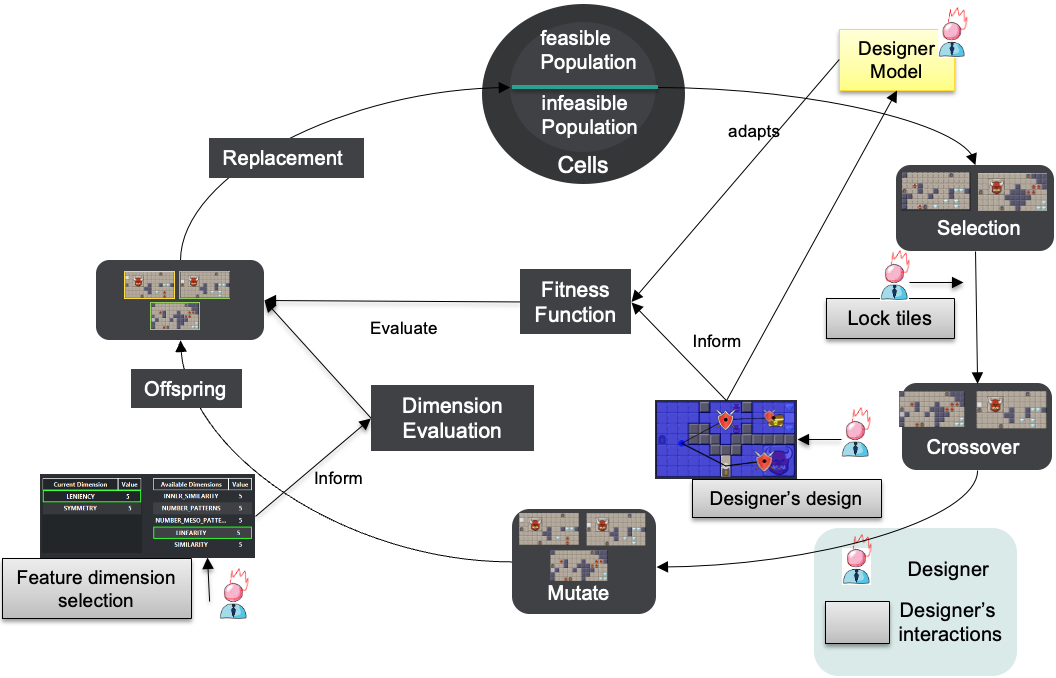
\includegraphics[width=\textwidth]{figures/EDD-figs/all-designers-interactions.png}}
\caption{\acrshort{icmape} evolutionary loop showing the possible designer interactions and what part of the loop these interaction affect} \label{fig:interactiveMAPE}
\end{figure}



% \subsubsection{Macro-patterns}

\subsection{Room Generation}

The main feature of~\acrshort{edd} is to suggest variations of the designer's work adapted to their design, are interesting, and can foster the designer's creativity. Through this, we seek that~\acrshort{edd} ends representing the role of a colleague, as discussed by Lubart~\cite{lubart_how_2005}. The suggestions have the main characteristic: they use the designer's current room configuration as target ratios (e.g., the number of corridors, the number of inventorial patterns, etc.) to provide adaptive suggestions. However, due to the algorithm's nature, the designer is also suggested content that respects these ratios but might use them differently with a different goal.

For instance, if the designer is creating a room with many corridors, such as a labyrinth, they will be provided with suggestions with a similar distribution of corridors, but utilizing the rest of space in different ways, as shown in figure~\ref{fig:corridorExample}.

\acrshort{edd} uses the~\acrshort{icmape} (explained in detail in section~\ref{sec:icmap-elites}) to generate and suggest rooms to the designer. Its main features are the use of divergent and convergent searches, the use of behavior feature dimensions, and the designer's ability to interact with them. Through this process,~\acrshort{edd} can provide a grid of evolved high-performing suggestions, adapted to the designer's current design, while representing a diverse set of solutions. For instance, in figure~\ref{fig:corridorExample}, it is shown multiple evolutionary runs when using the same design and the set of generated suggestions. It can be observed that the designer is provided with a set of suggestions that retained their expected ratios and design, but diverse enough that the designer can browse many different variations. It can also be observed the effect of the different feature dimensions, as some of them do not match the expected ratios adequately. Thus, producing bigger variations in the solutions to explore the search space. 

\begin{figure}[!h]
    \centering
     \subfloat[Example room]{%
       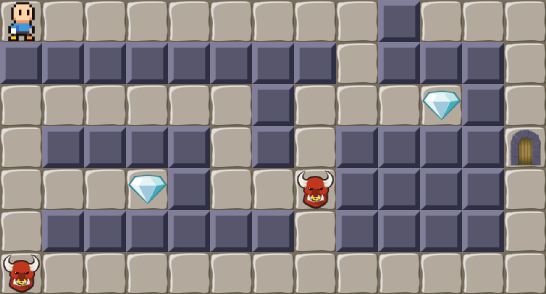
\includegraphics[width=0.48\textwidth]{figures/EDD-figs/corridor_example/currentRoom.png}
     }
     \hfill
     \subfloat[Design Patterns]{%
       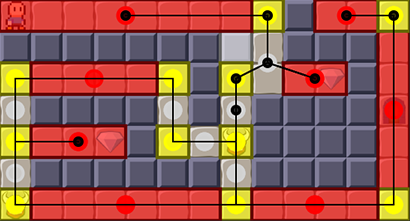
\includegraphics[width=0.48\textwidth]{figures/EDD-figs/corridor_example/room-corridors-final.png}
     }
     
      \subfloat[Meso-pattern and Leniency]{%
       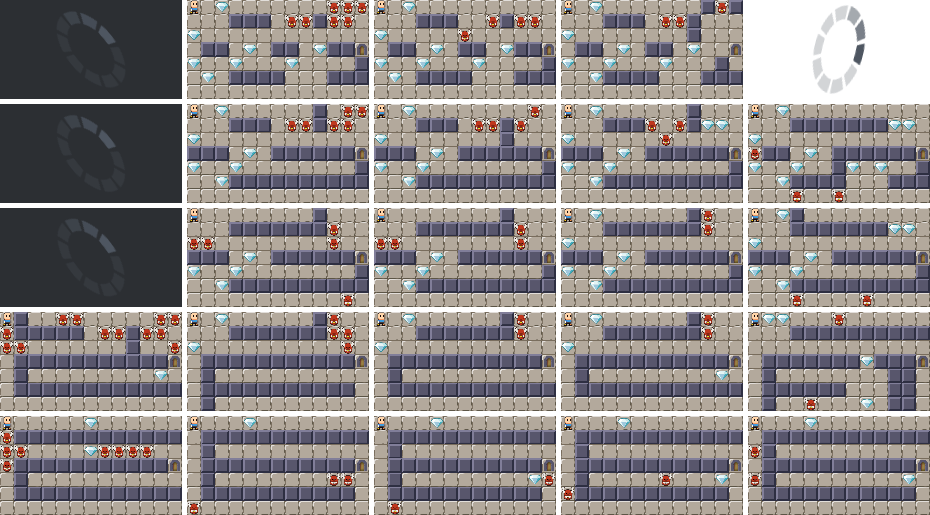
\includegraphics[width=0.48\textwidth]{figures/EDD-figs/corridor_example/meso-leniency-final.png}
     }
     \hfill
     \subfloat[Symmetry and Leniency]{%
       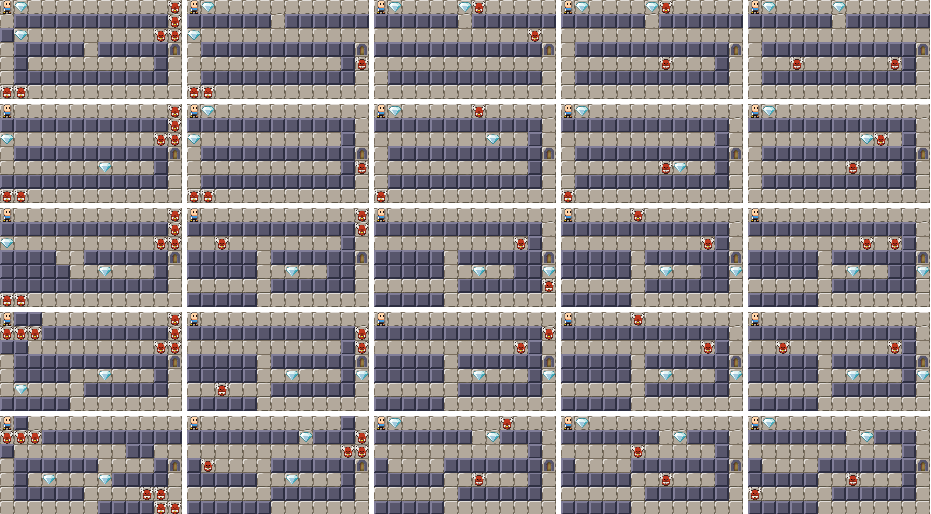
\includegraphics[width=0.48\textwidth]{figures/EDD-figs/corridor_example/sym-leniency-final.png}
     }
    
    \caption{Example of a possible room created by a designer (a), the design patterns identified by the system (b), and two suggestion grids presented to the designer (c and d). The rooms in both suggestion grids, were generated using~\acrshort{icmape} using respectively, \#meso-patterns and leniency (c), and symmetry and leniency (d) as dimensions.}
    \label{fig:corridorExample}
\end{figure}

\subsubsection{Evolutionary Components}

\acrshort{icmape} is an extension of the Constrained~\acrshort{mape}, which uses a~\acrshort{fi2pop} and~\acrshort{mape} at its core. In our implementation of~\acrshort{icmape}, a solution is deemed infeasible if the playability constraints are not satisfied, i.e., there is a passable tile that is not reachable from at least one door. If this happens, the solution is placed in the respective infeasible population to evolve into a feasible one encouraging diversity in the population.

Moreover,~\acrshort{edd} implements seven behavior feature dimensions (shown in table~\ref{table:mape-dimensions}). The designer can select one at a time, and only two dimensions can be active at any given time, in order to be able to present the suggestions intuitively to the designer and to focus the search on the pair of dimensions. By giving the designer this interaction, they can effectively reshape the search space of the~\acrshort{icmape}.

Furthermore, besides using feature dimensions to encounter diverse solutions,~\acrshort{edd} uses a single-objective fitness function to calculate the generated rooms' fitness. The fitness is a weighted sum divided equally between (1) the inventorial aspect of the rooms, which relates to the placement of enemies and treasures in relation to doors and target ratios, and (2) the spatial distribution of the design patterns, which refers to the distribution between corridors and rooms, and the meso-patterns that those encompass. The fitness adapts to the user's current design, automatically informing target ratios and distributions to be achieved by the~\acrshort{ea}.

The fitness function is shown in Eq.~\ref{fitness_func}. $f_{inventorial}$ is the evaluation of the aggregated and normalized quality of treasures, enemies, and doors (inventorial patterns). Quality refers to positioning, safety, and the relation between inventorial patterns. $f_{spatial}$ refers to the quality and distribution of chambers, i.e. open areas in the room and corridors, and the meso-patterns created within chambers. 

\begin{equation} 
\label{fitness_func}
f_{fitness}(r) = \frac{1}{2}f_{inventorial}(r) \,+ \, \frac{1}{2}f_{spatial}(r)
\end{equation}


% Cells are first created based on the dimensions selected by the user and proceed to initialize the population based on the user's design, evaluate it and assign each individual to the corresponding cell. Before starting each generation, we check if the dimensions have changed, and if so, recreate the cells and populate them with the previous individuals, and proceed through the evolutionary components. We first select uniformly random which cell to choose parents from, and then we select 5 parents through tournament-selection. Offspring are produced through a two-point uniform crossover operation with a 30\% chance of mutation. Offspring are placed in the correct cell and population after calculating their fitness and dimension's information. Finally, cells eliminate the low-performing individuals that over-cap their maximum capacity. Since interbreeding is not allowed, and can only happen indirectly (i.e. the offspring changing population and then used for breeding in consequent generations), the strategies are repeated for each of the populations.

% This procedure is repeated until the user decides to stop the algorithm. Meanwhile, the EA runs for $n$ generations, and once it reaches the specified limit, it broadcasts the found elites. In order to foster the exploration, we first mutate all the individuals from all the populations and cells (while retaining the previous population), and add them into the same pool together with the current edited room without changes. Finally, we evaluate and assign all the individuals to the correct cells, and cells that are over maximum capacity eliminates low-performing individuals.

% Selection is through competition, 

% That means that with a single run,~\acrshort{icmape} is able to generate a grid of solutions


% aligned to their and are interesting 

% The main feature of~\acrshort{edd} is the computational designer, which main task is to represent the role of a colleague as discussed by Lubart~\cite{LUBART2005-computerPartners}. In order to do this, 

% The formula for calculating the fitness score is the following: 

\subsubsection{Designer Interaction}
\label{sec:desInteraction}



One of the objectives of this thesis, and a significant feature in~\acrshort{edd}, is the control and interaction designers have with non-intuitive components of the algorithms. In~\acrshort{edd}, the designer can interact with the~\acrshort{icmape} in three different ways: 1) \emph{Locking tiles}: A special tile that locks tiles in the room to be unchangeable. 2) \emph{Feature dimensions}: The designer can change the feature dimensions of the~\acrshort{icmape} at any time, reshaping the search space. 3) \emph{Current design}: The designer is indirectly in constant interaction with the~\acrshort{icmape} by simply designing their room, which adapts the evaluation of generated solutions. 

% The designer can interact with the computational designer, and specifically with the~\acrshort{icmape} that generate the sugthrough

% Besides this, the designer can lock tiles 

% Whenever a designer chooses a suggestion, they are given some extra information 

\begin{figure}[!h]
\centerline{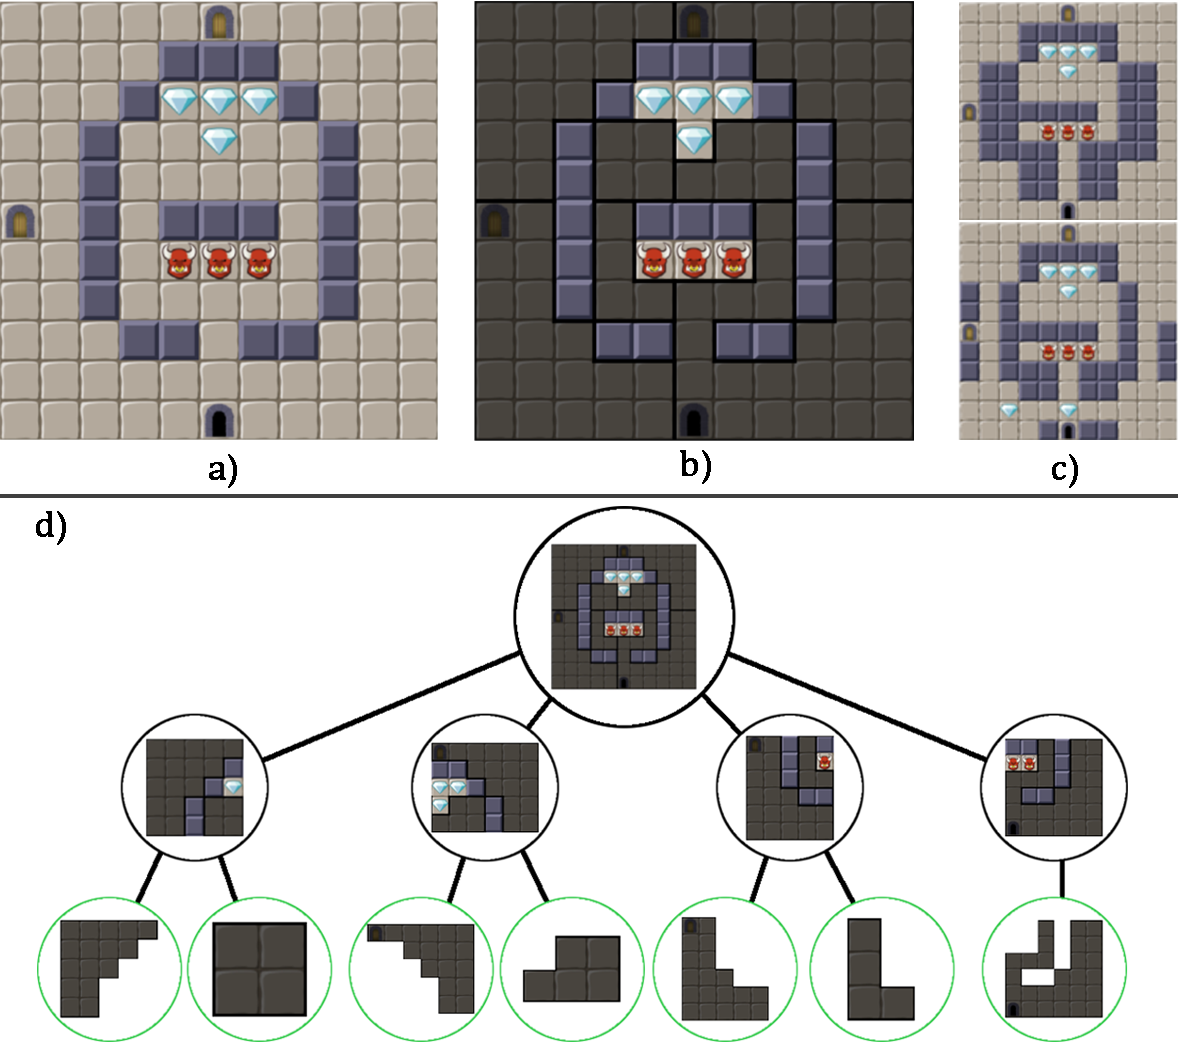
\includegraphics[width=0.8\textwidth]{figures/EDD-figs/map-representation-figure-test.png}}
\caption{Locking Tiles interaction: (a) A sample edited room with (b) its division into zones based on the tiles locked by the user.(c) Suggestions preserve these locked tiles. (d) The room and its zones are internally represented with a tree structure, where the leaf nodes (green) are the valid genes to apply variation operators.} \label{fig:lockTiles}
\end{figure}

\textbf{Locking tiles:} Besides the set of tiles provided to the designer to edit the room, they are given a modifier that allows them to lock tiles in their design, which establishes what tiles or structures must be preserved in the suggestions. By locking tiles, the designer is effectively constraining the building blocks~\acrshort{icmape} have for applying variation operators, as mutation and crossover will only happen on non-locked tiles. However, this also allows~\acrshort{icmape} to focus on the areas that the designer is not interested in, segmenting the room's design and promoting the colleague role. Figure~\ref{fig:lockTiles} shows an example of this interaction and how the genes are segmented in the~\acrshort{ea}.

% the designer is explicitly interacting with~\acrshort{icmape} by establishing what structures must be preserved in the suggestions.

\textbf{Feature Dimensions:} A major feature in~\acrshort{icmape} that differentiate the approach to other~\acrshort{mape} variations is the interaction designers have with the algorithm. Feature dimensions are an essential component of~\acrshort{mape}, used to discretizes the behavior space as a grid of cells, illuminating such space. Through this,~\acrshort{mape} can explore the space more vastly by retaining high-performing solutions in cells informed by the feature dimensions encountered in different parts of the behavior space. Furthermore, The designer can interact with these feature dimensions, choosing those of most interest to them. By doing this, the search and solutions encountered are conditioned to the designer's interest. Changing the dimensions reshapes the behavior characteristics where encountered individuals in the search space will be retained.

\textbf{Current Design:}~\acrshort{edd} uses an adaptive fitness function based on the designer's design by analyzing the room configuration based on the design patterns previously described. This allows the designer to interact indirectly with how~\acrshort{icmape} estimates the quality of the encountered solutions. Therefore, to achieve high-fitness, the generated content will need to have certain similar characteristics than the current design, in order for the content to do not be too disparate from the designer's goal. However, while this might limit the tool's expressivity,~\acrshort{icmape} use of feature dimensions and leverage on convergent and divergent searches still yields diverse solutions.

Finally, in figure~\ref{fig:interactiveMAPE}, it is presented an overview of the~\acrshort{icmape} steps and the multiple areas designers can interact.


% \subsubsection{Designer Modeling}

\subsection{Workflow}

\acrshort{edd} has three views that enable the~\acrshort{micc} wokflow depicted in figure~\ref{fig:eddWorkflow}.

\subsubsection{World View}

In figure~\ref{fig:eddWorkflow}(a), it is shown the world view. This view provides the designer with an overview of their dungeon while allowing them to create new rooms and edit their connections. The dungeon is a cyclical graph in code, which allows the needed flexibility for the designer to create whatever layout they want. The designer can create or delete any number of rooms and can connect them as needed. By editing these connections, they edit the rooms' entrance and exit doors, effectively changing the layout and gameplay flow. For instance, the designer can create linear gameplay with rooms one after the other, or gameplay that rewards exploration through dead-ends with some side-objective. 

To edit a room, the designer can: 1) double-click or scroll to zoom-in any room to change the view to the \emph{room view} or 2) select a room and click the ``Suggestions'' button, which will take them to the \emph{suggestion view}

\subsubsection{Suggestion View}

In this view (shown in figure~\ref{fig:eddWorkflow}(b)), the designer is proposed six variations to their design based on six different preset room configuration: Favoring open areas, favoring corridors, a mix of open areas and corridors, favoring dead-ends, favoring meso-patterns, and using the actual room configuration. The designer can then go back to the world view or choose any of the suggestions and start editing their room using that as a base in the \emph{room view}.

\subsubsection{Room View}

The room view (shown in figure~\ref{fig:eddWorkflow}(c)) is the main view in~\acrshort{edd}, where both the designer and the computational designer interact to co-create rooms. As mentioned above, the designer has five different tiles at their disposal to create a room that fulfills their objective. Besides this, the designer can enable the ``patterns visualization'' that overlays on the designer's design what spatial- and meso-patterns are identified.

\acrshort{edd} incorporates a feasibility and playability check on the designer's design. This informs the designer if an area in the room is inaccessible from within the room or through another room by adding a red border in their design and an information box. This feasibility check is reused in the~\acrshort{ea} used by the computational designer to generate suggestions for the designer. 

Moreover, in this view, the designer edits the room as they want, while on the right side of the view, they are suggested a collection of rooms. Whenever a suggestion is selected, a quantitative comparison between the suggestion and the current design is presented to the designer. If the designer decides to replace their design with the suggestion, they apply it and continue the design process. The system aims to give suggestions to the designer that are interesting for them, aligned with their current design, but at the same time different enough to foster their creativity. Designers might not apply any suggestion, but a designer might be interested in doing something similar by observing them. 

Once the designer finishes editing their room, they can go back to the world view and start another room's design process until they finish their dungeon. 

\begin{figure}[!h]
\centerline{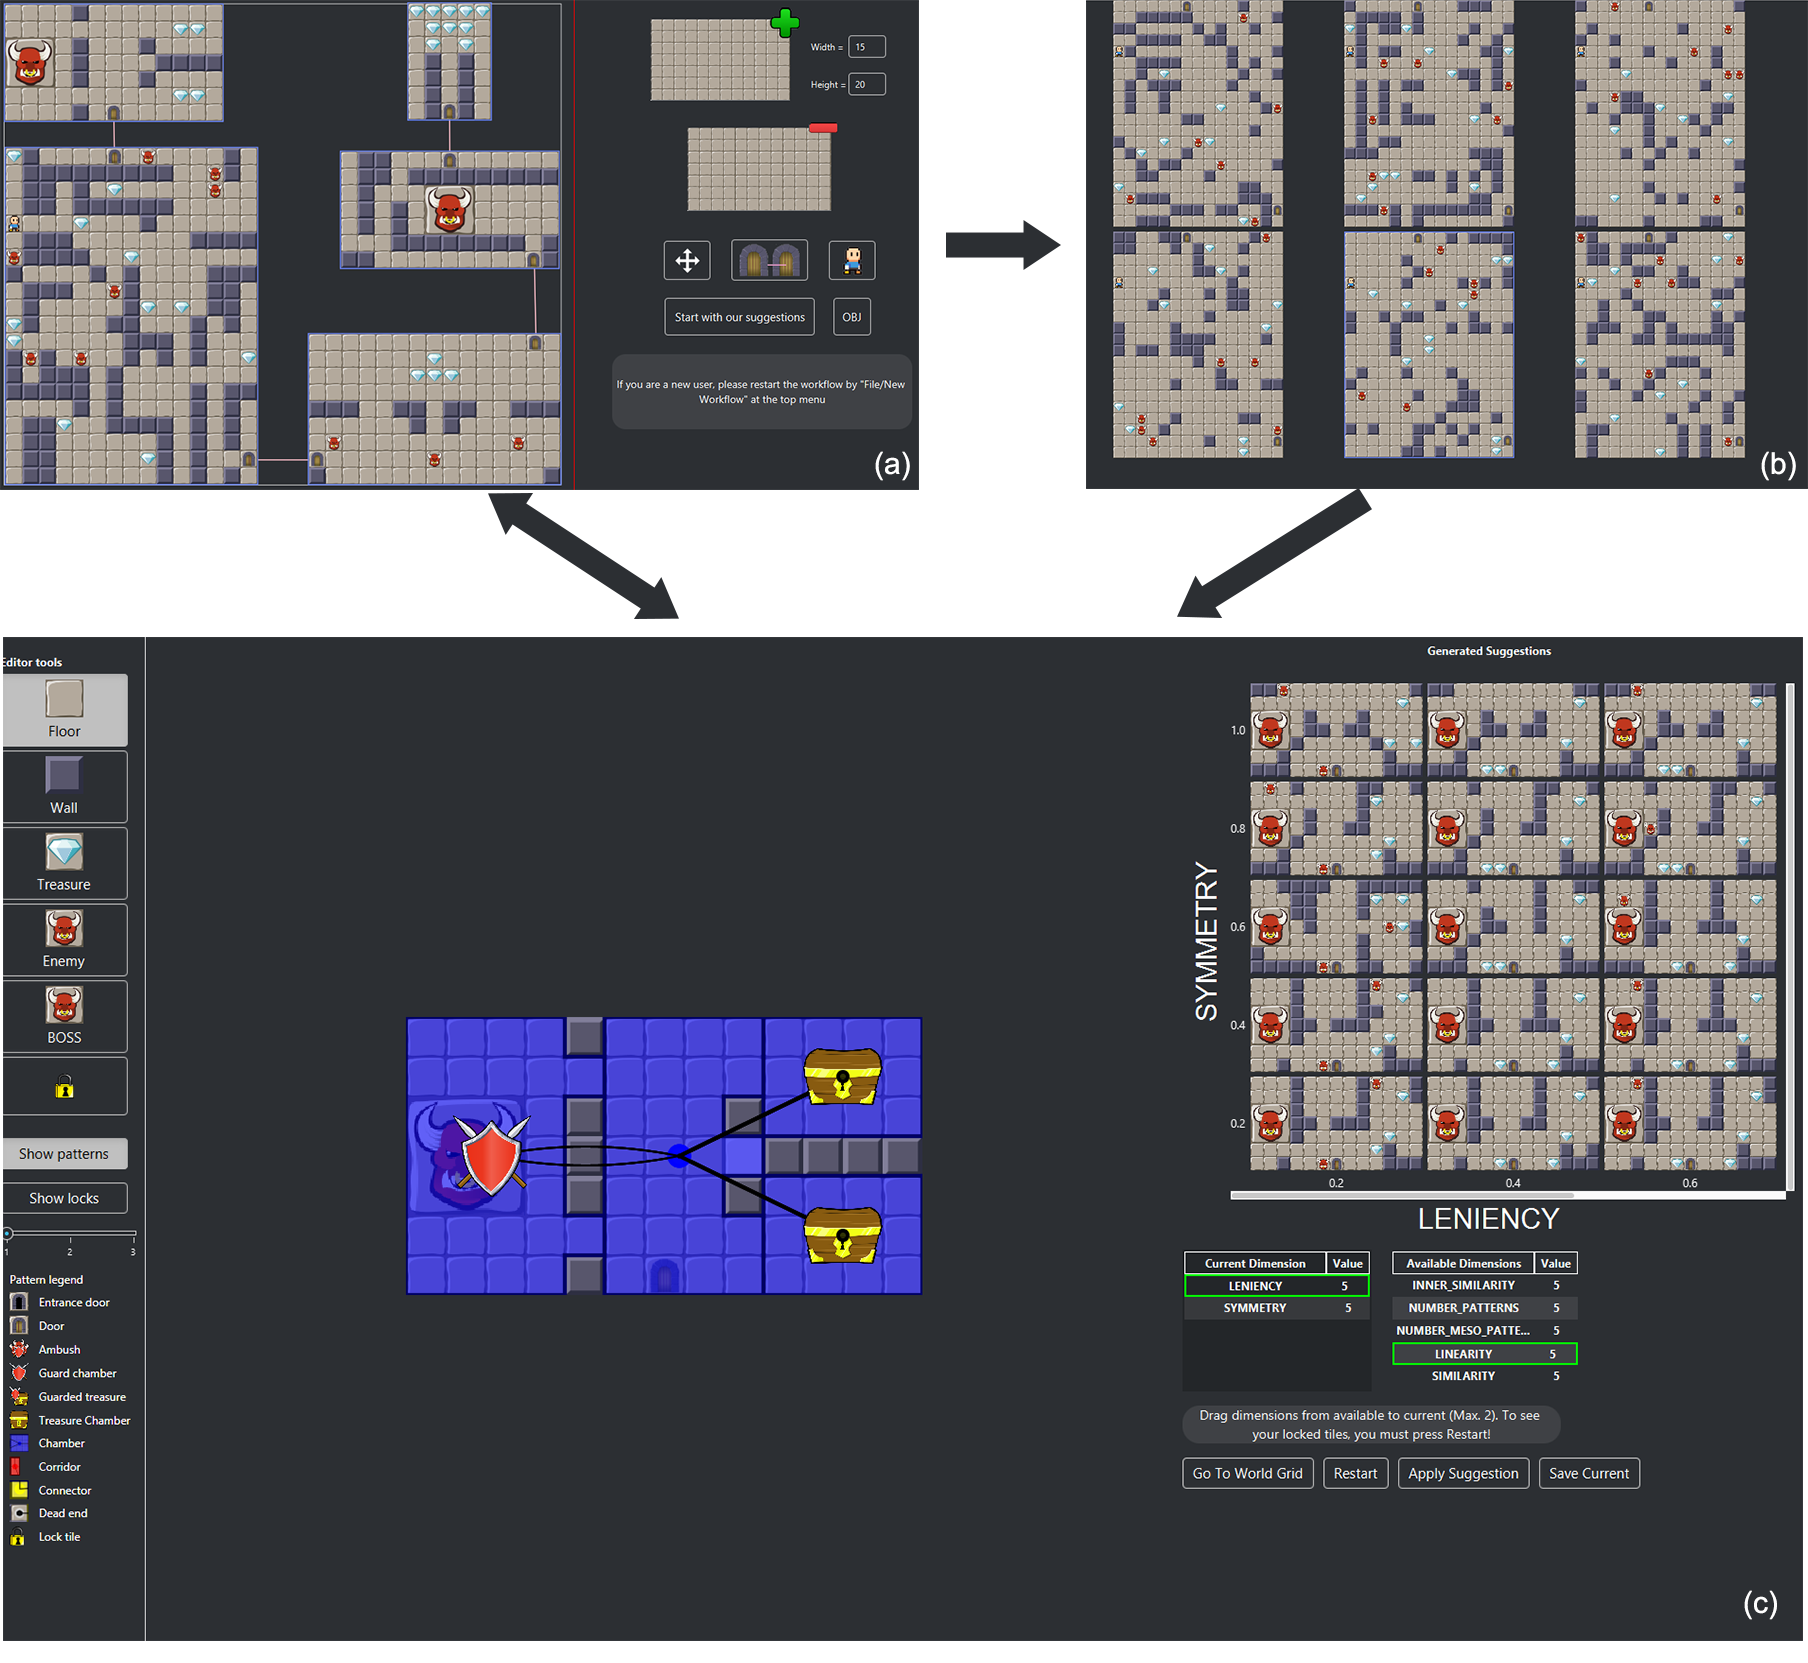
\includegraphics[width=\textwidth]{figures/EDD-figs/edd-workflow-2.png}}
\caption{Workflow of the~\acrlong{edd}. (a) Shows the world view with a prototype dungeon created. (b) Shows the suggestion view where designers can receive instantly six suggestions to start their design with, rather than from scratch. (c) Shows the room view, the main interactive view of~\acrshort{edd}. In this view the designer can edit their room while the computational designer is offering suggestions for their design.} \label{fig:eddWorkflow}
\end{figure}



% These rooms can be examined


% when their design do not fulfill the requirements. These are: 1) there is an area in the room that is inaccessible from within the room or through another room

% As the designer creates their room, the system is constantly 




% In~\acrshort{edd} the designer can create individuals rooms of different sizes and interconnect them to compose dungeons with different types of gameplay. 

